% cd /storage/emulated/0/Documents/documents/latex/1920/Grade-10/1st/radii-and-chords && pdflatex ps-radii-and-chords.tex && termux-open ps-radii-and-chords.pdf

% cd /storage/emulated/0/Documents/documents/latex/1920/Grade-10/1st/radii-and-chords && clean-tex ps-radii-and-chords-input1.tex


% cd /storage/emulated/0/Documents/documents/latex/1920/Grade-10/1st/radii-and-chords && convert -density 600 ps-radii-and-chords.pdf -crop 2200x1700 -quality 100 -verbose ps-radii-and-chords%02d.png

%2480.5x3508 portrait 2x2 2550x3300
%3508x2480.5 landscape 2x2 3300x2550 
%1653.7x2338.7 portrait 3x3 1700x2200
%landscape 3x3 2200x1700

% cd /storage/emulated/0/Documents/documents/latex/1819/grade10/visual/4th/radii-and-chords && while inotifywait -e close_write ps-radii-and-chords*.tex; do touch /storage/emulated/0/Android/data/com.termux/files/launch-termux.txt && printf '1' > /storage/emulated/0/Android/data/com.termux/files/launch-termux.txt && pdflatex ps-radii-and-chords.tex && termux-open ps-radii-and-chords.pdf; done

% cd /host-rootfs/storage/emulated/0/Documents/documents/latex/1819/grade10/visual/4th/radii-and-chords && while inotifywait -e close_write ps-radii-and-chords*.tex; do pdflatex ps-radii-and-chords.tex  && printf "/storage/emulated/0/Documents/documents/latex/1819/grade10/visual/4th/radii-and-chords/ps-radii-and-chords.pdf" > /host-rootfs/storage/emulated/0/GNURoot/home/Scripts/file-to-launch.txt; done


\documentclass[10pt]{article}
\usepackage[letterpaper, landscape, right=0.25in, left=0.25in, top=0.25in, bottom=0.25in]{geometry}
\usepackage{xcolor}
\usepackage{anyfontsize}
\usepackage{enumitem}
\usepackage{multicol}
\usepackage{amsmath}
%\usepackage{amsfonts,dsfont}% for \mathds 
\usepackage{tabularx} 
\usepackage{gensymb}
\usepackage{multirow}
\usepackage{graphicx, tipa}
\usepackage{tikz}
\usetikzlibrary{angles,quotes}
\usepackage{pgfplots} 
\usetikzlibrary{calc}
\pgfplotsset{compat=newest}
\usetikzlibrary{arrows.meta}
\usetikzlibrary{intersections}
\usetikzlibrary{decorations.pathreplacing}
\usepackage{flafter}
\usepackage{amsmath,amssymb,cancel,units}
\usepackage{microtype} % nicer output 
\usepackage{hfoldsty} % nicer output 
\usepackage{fixltx2e} 
\usepackage{mathptmx}
%\usepackage{booktabs}
\usepackage{numprint}
\usepackage[utf8]{inputenc} 
\usepackage[T1]{fontenc}
%\usepackage{siunitx} 
%\sisetup{detect-all}


\def\radA{3.6cm}

\def\radB{3.6cm}

%\def\thirdrad{8cm}

\pagenumbering{gobble}
%\linespread{0.9}
\newcommand{\vspce}{\vspace{0.75ex}}
\newcommand{\hspce}{\hspace{0.5em}}
\newcommand{\blank}{\underline{\hspace{2em}}}%{\rule{1em}{0.15ex}}
\newcommand{\arc}[1]{{% 
\setbox9=\hbox{#1}% 
\ooalign{\resizebox{\wd9}{\height}{\texttoptiebar{\phantom{A}}}\cr#1}}}

\newcolumntype{C}{ >{\centering\arraybackslash} X}




\begin{document}
\boldmath
{\fontsize{36}{40}\fontfamily{pnc}\selectfont {

\def\currentdir{/storage/emulated/0/Documents/documents/latex/1920/Grade-10/2nd/radii-and-chords}

\textbf{Practice Exercises}

\vspace*{-2ex}

\begin{center}
\scalebox{1}{
\noindent\begin{minipage}{\textwidth}
{
A. In $\odot{I}$, $\overline{PH}$ and $\overline{CE}$ are diameters with $\overline{PH}\perp\overline{AE}$ and $\overline{PH}\perp\overline{CU}$. 

\begin{enumerate}[label = \arabic*. ]
\item Name the midpoint of $\overline{PH}$. 
\item Name the midpoint of $\overline{CE}$.
\item Name the midpoint of $\overline{AE}$. %\hspace*{6cm}\vspace*{0ex}
\begin{tikzpicture}[dot/.style={circle, fill=black, inner sep=0pt, outer sep=0pt, minimum size=4pt},
nodot/.style={circle, fill=black, inner sep=0pt, outer sep=0pt, minimum size=0pt},
 remember picture, overlay
]

\def\radfig1{1.5cm}

\node(i)[dot] at (0,0) {};

\draw[name path=circ, line width=0.4mm] (i) circle (\radfig1);

\node(i-label) at ($(i)+(120:0.18*\radfig1)$) {$\  I$};

\coordinate (p) at ($(i) +(180:\radfig1)$);

\node(p-label) at ($(p)+(180:0.22*\radfig1)$) {$\  P$};

\coordinate (h) at ($(i) +(0:\radfig1)$);

\node(h-label) at ($(h)+(0:0.1*\radfig1)$) {$\  H$};

\node[nodot] (w) at ($(p)!0.5!(i)$){};

\node(w-label) at ($(w)+(145:0.25*\radfig1)$) {$\  W$};

\node[nodot] (n) at ($(i)!0.5!(h)$){};

\node(n-label) at ($(n)+(60:0.15*\radfig1)$) {$\  N$};

\path[name path=line1.guess, line width=0.5mm] (n) -- ($(n)!3!-90:(i)$);

\fill[black, name intersections={of=line1.guess and circ, name=point}];

\node[nodot] (c) at (point-1){};

\node(c-label) at ($(c)+(90:0.22*\radfig1)$) {$\  C$};

\path[name path=line2.guess, line width=0.5mm] (n) -- ($(n)!3!90:(i)$);

\fill[black, name intersections={of=line2.guess and circ, name=point}];

\node[nodot] (u) at (point-1){};

\node(u-label) at ($(u)+(-90:0.22*\radfig1)$) {$\  U$};

\path[name path=line3.guess, line width=0.5mm] (w) -- ($(w)!3!90:(i)$);

\fill[black, name intersections={of=line3.guess and circ, name=point}];

\node[nodot] (a) at (point-1){};

\node(a-label) at ($(a)+(110:0.22*\radfig1)$) {$\  A$};

\path[name path=line4.guess, line width=0.5mm] (w) -- ($(w)!3!-90:(i)$);

\fill[black, name intersections={of=line4.guess and circ, name=point}];

\node[nodot] (e) at (point-1){};

\node(e-label) at ($(e)+(-120:0.22*\radfig1)$) {$\  E$};

\draw[line width=0.5mm] (p) -- (h);

\draw[line width=0.5mm] (a) -- (e);

\draw[line width=0.5mm] (e) -- (c);

\draw[line width=0.5mm] (c) -- (u);


\end{tikzpicture}
\vspace*{-1.5ex}
\item Name the midpoint of $\overline{CU}$.
\item If $\overline{IW}\cong\overline{IN}$, name a chord  congruent \newline
 to $\overline{AE}$ and an arc  congruent to $\arc{CHU}$. 
\item Name two arcs congruent to $\arc{AP}$. 
\end{enumerate}  
\vspace*{-2.5cm}\hspace*{8.5cm}
\begin{tikzpicture}[dot/.style={circle, fill=black, inner sep=0pt, outer sep=0pt, minimum size=4pt},
nodot/.style={circle, fill=black, inner sep=0pt, outer sep=0pt, minimum size=0pt},
 remember picture, overlay
]

\def\radfig1{1.5cm}

\node(i)[dot] at (0,0) {};

\draw[name path=circ, line width=0.4mm] (i) circle (\radfig1);

\node(i-label) at ($(i)+(120:0.18*\radfig1)$) {$\  I$};

\coordinate (p) at ($(i) +(180:\radfig1)$);

\node(p-label) at ($(p)+(180:0.22*\radfig1)$) {$\  P$};

\coordinate (h) at ($(i) +(0:\radfig1)$);

\node(h-label) at ($(h)+(0:0.1*\radfig1)$) {$\  H$};

\node[nodot] (w) at ($(p)!0.5!(i)$){};

\node(w-label) at ($(w)+(145:0.25*\radfig1)$) {$\  W$};

\node[nodot] (n) at ($(i)!0.5!(h)$){};

\node(n-label) at ($(n)+(60:0.15*\radfig1)$) {$\  N$};

\path[name path=line1.guess, line width=0.5mm] (n) -- ($(n)!3!-90:(i)$);

\fill[black, name intersections={of=line1.guess and circ, name=point}];

\node[nodot] (c) at (point-1){};

\node(c-label) at ($(c)+(90:0.22*\radfig1)$) {$\  C$};

\path[name path=line2.guess, line width=0.5mm] (n) -- ($(n)!3!90:(i)$);

\fill[black, name intersections={of=line2.guess and circ, name=point}];

\node[nodot] (u) at (point-1){};

\node(u-label) at ($(u)+(-90:0.22*\radfig1)$) {$\  U$};

\path[name path=line3.guess, line width=0.5mm] (w) -- ($(w)!3!90:(i)$);

\fill[black, name intersections={of=line3.guess and circ, name=point}];

\node[nodot] (a) at (point-1){};

\node(a-label) at ($(a)+(110:0.22*\radfig1)$) {$\  A$};

\path[name path=line4.guess, line width=0.5mm] (w) -- ($(w)!3!-90:(i)$);

\fill[black, name intersections={of=line4.guess and circ, name=point}];

\node[nodot] (e) at (point-1){};

\node(e-label) at ($(e)+(-120:0.22*\radfig1)$) {$\  E$};

\draw[line width=0.5mm] (p) -- (h);

\draw[line width=0.5mm] (a) -- (e);

\draw[line width=0.5mm] (e) -- (c);

\draw[line width=0.5mm] (c) -- (u);


\end{tikzpicture}
\vspace*{2.5cm}
}
\end{minipage}}
\end{center} 


%}} 

%\newpage

%{\fontsize{38}{40}\fontfamily{pnc}\selectfont {

\def\currentdir{/storage/emulated/0/Documents/documents/latex/1920/Grade-10/2nd/radii-and-chords}

\begin{center}
\vspace*{-2ex}
\scalebox{1}{
\noindent\begin{minipage}{\textwidth}
{
B. In $\odot{T}$, $\overline{AT}$ is a radius and $\overline{AL}$ is a chord. 
\begin{enumerate}[label = \arabic*. ]

\item If $\overline{TK}\perp\overline{AL}$, then $\overline{TK}\blank\overline{AL}$. 
\item If $\overrightarrow{TK}$ bisects $\angle{ATL}$, then  $\overrightarrow{TK}\blank\overline{AL}$. 
\item If $\overline{TK}$ is a perpendicular  bisector \newline of $\overline{AL}$, then $\overrightarrow{TK}\blank\angle{ATL}$. 
\item The altitude $\overrightarrow{TK}$ to the base of \newline $\Delta{ATL}$ is also a \blank. 
\end{enumerate}  
\vspace*{-2.8cm}\hspace*{8.5cm}\begin{tikzpicture}[dot/.style={circle, fill=black, inner sep=0pt, outer sep=0pt, minimum size=4pt},
nodot/.style={circle, fill=black, inner sep=0pt, outer sep=0pt, minimum size=0pt},
 remember picture, overlay
]

\def\radfig2{1.5cm}

\node(t)[dot] at (0,0) {};

\draw[name path=circ, line width=0.5mm] (t) circle (\radfig2);

\node(t-label) at ($(t)+(180:0.22*\radfig2)$) {$\  T$};

\coordinate (b) at ($(t) +(0:\radfig2)$);

\node[nodot] (k) at ($(t)!0.5!(b)$){};

\node(k-label) at ($(k)+(45:0.22*\radfig2)$) {$\  K$};

\path[name path=line.guess, line width=0.5mm] (k) -- ($(k)!3!-90:(t)$);

\fill[black, name intersections={of=line.guess and circ, name=point}];

\node[nodot] (a) at (point-1){};

\node(a-label) at ($(a)+(70:0.22*\radfig2)$) {$\  A$};

\path[name path=line2.guess, line width=0.5mm] (k) -- ($(k)!3!90:(t)$);

\fill[black, name intersections={of=line2.guess and circ, name=point}];

\node[nodot] (l) at (point-1){};

\node(l-label) at ($(l)+(-90:0.22*\radfig2)$) {$\  L$};

\draw[line width=0.5mm] (a) -- (t);

\draw[line width=0.5mm, ->, >={Latex[round]}] (t) -- ($(t)!1.3!(b)$);

\draw[line width=0.5mm] (a) -- (l) -- (t) ;

%\node(figure2) at ($(t)+(-90:1.3*\radfig2)$) {\LARGE Figure for Nos. 7--10};

\end{tikzpicture}

\vspace*{2.8cm}
}
\end{minipage}}
\end{center} 
}}
\newpage

{\fontsize{36}{40}\fontfamily{pnc}\selectfont {
\def\radfig3a{1.5cm}
\def\currentdir{/storage/emulated/0/Documents/documents/latex/1920/Grade-10/2nd/radii-and-chords}

\textbf{Problem Set}

\vspce

Find the value of $x$ in each figure. 

\begin{center}
\scalebox{1}{
\noindent\begin{minipage}{\textwidth}
{\begin{tabularx}{\textwidth}{XX}

1. \begin{tikzpicture}[dot/.style={circle, fill=black, inner sep=0pt, outer sep=0pt, minimum size=3pt}, 
nodot/.style={circle, fill=black, inner sep=0pt, outer sep=0pt, minimum size=0pt}, 
%remember picture,% overlay
baseline = (current bounding box.west)
]  

\node(i)[dot] at (0,0) {};

\draw[name path=circ, line width=0.5mm] (i) circle (\radfig3a);

\coordinate (f) at ($(i) +(\radfig3a, 0)$);

\coordinate (g) at ($(i) -(\radfig3a, 0)$);

\coordinate (int1) at ($(i)! 0.66!(f)$);

\coordinate (int2) at ($(i)! 0.66!(g)$);

\coordinate (tick1) at ($(i)! 0.33!(f)$);

\coordinate (tick2) at ($(i)! 0.33!(g)$);

\draw[line width=0.3mm] ($(tick1)+(0,0.1*\radfig3a)$) -- ($(tick1)-(0,0.1*\radfig3a)$);

\draw[line width=0.3mm] ($(tick2)+(0,0.1*\radfig3a)$) -- ($(tick2)-(0,0.1*\radfig3a)$); 

\node(x.label) at ($(int1)+(30:0.13*\radfig3a)$) {$x$};

\node(12-label) at ($(int2)+(150:0.22*\radfig3a)$) {$12$};

\path[name path=line1.guess, line width=0.5mm] (int1) -- ($(int1)!3!90:(i)$);

\fill[black, name intersections={of=line1.guess and circ, name=point}];

\node[nodot] (d) at (point-1){};

\node(d-label) at ($(d)+(-60:0.22*\radfig3a)$) {$\  D$};

\path[name path=line2.guess, line width=0.5mm] (int1) -- ($(int1)!3!-90:(i)$);

\fill[black, name intersections={of=line2.guess and circ, name=point}];

\node[nodot] (c) at (point-1){};

\node(c-label) at ($(c)+(60:0.22*\radfig3a)$) {$\  C$};

\path[name path=line3.guess, line width=0.5mm] (int2) -- ($(int2)!3!90:(i)$);

\fill[black, name intersections={of=line3.guess and circ, name=point}];

\node[nodot] (a) at (point-1){};

\node(a-label) at ($(a)+(120:0.22*\radfig3a)$) {$\  A$};

\path[name path=line4.guess, line width=0.5mm] (int2) -- ($(int2)!3!-90:(i)$);

\fill[black, name intersections={of=line4.guess and circ, name=point}];

\node[nodot] (b) at (point-1){};

\node(b-label) at ($(b)+(240:0.22*\radfig3a)$) {$\  B$};

\draw[line width=0.5mm] (int2) -- (int1) ;

\draw[line width=0.5mm] (c) -- (d) ;

\draw[line width=0.5mm] (a) -- (b) ;

\begin{scope} [rotate=180]
\draw[line width=0.3mm] (int1) rectangle ++(0.22*\radfig3a,0.22*\radfig3a) node[transform shape]{};
\end{scope}

\begin{scope} [rotate=0]
\draw[line width=0.3mm] (int2) rectangle ++(0.22*\radfig3a,0.22*\radfig3a) node[transform shape]{};
\end{scope}

\end{tikzpicture}

  & 5. \begin{tikzpicture}[dot/.style={circle, fill=black, inner sep=0pt, outer sep=0pt, minimum size=3pt}, 
%dim-label/.style={fill=white, rectangle, inner sep=2pt, outer sep=0pt}, 
nodot/.style={circle, fill=black, inner sep=0pt, outer sep=0pt, minimum size=0pt}, 
%remember picture, overlay, 
baseline = (current bounding box.west)
] 

\node(i)[dot] at (0,0) {};

\draw[name path=circ, line width=0.5mm] (i) circle (\radfig3a);

\coordinate (a) at ($(i) + (100:\radfig3a)$);

\coordinate (b) at ($(i) + (220:\radfig3a)$);

\coordinate (c) at ($(i) + (340:\radfig3a)$);

\coordinate (int) at ($(a)! 0.5!(c)$);

\node(a.label) at ($(a)+(100:0.22*\radfig3a)$) {$  A$};

\node(b.label) at ($(b)+(220:0.22*\radfig3a)$) {$  B$};

\node(c.label) at ($(c)+(340:0.22*\radfig3a)$) {$  C$};

\node(x.label) at ($(int)+(40:0.13*\radfig3a)$) {$  x$};

\pic [draw, line width=0.3mm, angle radius=0.25*\radfig3a] {angle=b--a--c};

\pic [draw, line width=0.3mm, angle radius=0.25*\radfig3a] {angle=a--c--b};

\pic [draw, line width=0.3mm, angle radius=0.25*\radfig3a] {angle=c--b--a};
 
\draw[line width=0.3mm] ($(a)! 0.15*\radfig3a! (i) $) -- ($(a)! 0.35*\radfig3a! (i) $) ;

\draw[line width=0.3mm] ($(b)! 0.15*\radfig3a! (i) $) -- ($(b)! 0.35*\radfig3a! (i) $) ;

\draw[line width=0.3mm] ($(c)! 0.15*\radfig3a! (i) $) -- ($(c)! 0.35*\radfig3a! (i) $) ;

\draw[line width=0.5mm] (a) -- (b) node[midway, xshift=-0.22*\radfig3a] (17.label) {$17$};;

\draw[line width=0.5mm] (c) -- (b) ;

\draw[line width=0.5mm] (a) -- (c) ;

\draw[line width=0.3mm, densely dotted] (b) -- (int) ;

\begin{scope} [rotate=-140]
\draw[line width=0.3mm] (int) rectangle ++(0.22*\radfig3a,0.22*\radfig3a) node[transform shape]{};
\end{scope}

\end{tikzpicture}

\\
2. \begin{tikzpicture}[dot/.style={circle, fill=black, inner sep=0pt, outer sep=0pt, minimum size=3pt}, 
nodot/.style={circle, fill=black, inner sep=0pt, outer sep=0pt, minimum size=0pt}, 
%remember picture, overlay, 
baseline = (current bounding box.west)
]  

\node(i)[dot] at (0,0) {};

\draw[name path=circ, line width=0.5mm] (i) circle (\radfig3a);

\coordinate (b) at ($(i) +(120:\radfig3a)$);

\node(b-label) at ($(b)+(120:0.22*\radfig3a)$) {$\  B$};

\coordinate (c) at ($(i) +(70:\radfig3a)$);

\node(c-label) at ($(c)+(70:0.22*\radfig3a)$) {$\  C$};

\coordinate (e) at ($(i) +(250:\radfig3a)$);

\node(e-label) at ($(e)+(250:0.22*\radfig3a)$) {$E$};

\coordinate (int1) at ($(i)! 0.66!(e)$);

\path[name path=line.guess, line width=0.5mm] ($(int1)!2!-90:(i)$) -- ($(int1)!2!90:(i)$);

\fill[black, name intersections={of=line.guess and circ, name=point}];

\node[nodot] (a) at (point-1){};

\node[nodot] (d) at (point-2){};

\node(a-label) at ($(a) +(160:0.22*\radfig3a)$) {$\  A$};

\node(d-label) at ($(d) +(-20:0.22*\radfig3a)$) {$\  D$};

\node(50-label) at ($(int1) +(200:0.8*\radfig3a)$) {$\  50\degree$};

\node(x.label) at ($(int1) +(-60:0.6*\radfig3a)$) {$x$};

\draw[line width=0.3mm] (a) -- (d) ;

\draw[line width=0.3mm] (c) -- (e) ;

\draw[line width=0.3mm] (i) -- (b) ;

\begin{scope} [rotate=160]
\draw[line width=0.3mm] (int1) rectangle ++(0.22*\radfig3a,0.22*\radfig3a) node[transform shape]{};
\end{scope}

\end{tikzpicture}

  & 6. \begin{tikzpicture}[dot/.style={circle, fill=black, inner sep=0pt, outer sep=0pt, minimum size=3pt}, 
%dim-label/.style={fill=white, rectangle, inner sep=2pt, outer sep=0pt}, 
nodot/.style={circle, fill=black, inner sep=0pt, outer sep=0pt, minimum size=0pt}, 
%remember picture, overlay, 
baseline = (current bounding box.west)
] 

\node(c)[dot] at (0,0) {};

\draw[name path=circ, line width=0.5mm] (c) circle (\radfig3a);

\node(c-label) at ($(c)+(225:0.22*\radfig3a)$) {$\  C$};

\coordinate (a) at ($(i) + (0, \radfig3a)$);

\coordinate (b) at ($(i) +(\radfig3a, 0)$);

\coordinate (int) at ($(a)! 0.5!(b)$);

\node(a.label) at ($(a)+(90:0.22*\radfig3a)$) {$\  A$};

\node(b.label) at ($(b)+(0:0.19*\radfig3a)$) {$B$};

\draw[line width=0.3mm] (a) -- (c) node [midway, xshift=-0.12*\radfig3a] (6.label) {$6$} -- (b) ;

\draw[line width=0.3mm] (a) -- (b) node [midway, xshift=0.11*\radfig3a, yshift=0.09*\radfig3a] (x.label) {$x$};

\draw[line width=0.3mm] (c) -- (int) ;

\begin{scope} [rotate=135]
\draw[line width=0.3mm] (int) rectangle ++(0.22*\radfig3a,0.22*\radfig3a) node[transform shape]{};
\end{scope}

\begin{scope} [rotate=0]
\draw[line width=0.3mm] (c) rectangle ++(0.22*\radfig3a,0.22*\radfig3a) node[transform shape]{};
\end{scope}

\end{tikzpicture}

\\
3. \begin{tikzpicture}[dot/.style={circle, fill=black, inner sep=0pt, outer sep=0pt, minimum size=3pt}, 
%dim-label/.style={fill=white, rectangle, inner sep=2pt, outer sep=0pt}, 
nodot/.style={circle, fill=black, inner sep=0pt, outer sep=0pt, minimum size=0pt}, 
%remember picture, overlay, 
baseline = (current bounding box.west)
] 

\node(o)[dot] at (0,0) {};

\draw[name path=circ, line width=0.5mm] (o) circle (\radfig3a);

\node(o-label) at ($(o)+(170:0.22*\radfig3a)$) {$  O$};

\coordinate (c) at ($(o) -(0,\radfig3a)$);

\node(c.label) at ($(c)+(-90:0.22*\radfig3a)$) {$  C$};

\coordinate (d) at ($(o) +(0,\radfig3a)$);

\node(d.label) at ($(d)+(90:0.22*\radfig3a)$) {$  D$};

\coordinate (e) at ($(o) +(50:\radfig3a)$);

\node(e.label) at ($(e)+(50:0.22*\radfig3a)$) {$  E$};

\coordinate (int1) at ($(o)! 0.55!(c)$);

\path[name path=line.guess, line width=0.5mm] ($(int1)!2!-90:(i)$) -- ($(int1)!2!90:(i)$);

\fill[black, name intersections={of=line.guess and circ, name=point}];

\node[nodot] (a) at (point-1){};

\node(a-label) at ($(a)+(180:0.22*\radfig3a)$) {$  A$};

\node[nodot] (b) at (point-2){};

\node(b.label) at ($(b)+(0:0.22*\radfig3a)$) {$  B$};

\draw[line width=0.3mm] (c) -- (d) ;

\draw[line width=0.3mm] (a) -- (b) ;

\draw[line width=0.3mm] (o) -- (e) node[midway, xshift=0.15*\radfig3a, yshift=-0.2*\radfig3a] (8.4.label) {$  8.4$};

\begin{scope} [rotate=0]
\draw[line width=0.3mm] (int1) rectangle ++(0.22*\radfig3a,0.22*\radfig3a) node[transform shape]{};
\end{scope}

\coordinate (tick1) at ($(int1)!0.5!(a)$);

\coordinate (tick2) at ($(int1)!0.5!(b)$);

\draw[line width=0.3mm] ($(tick1)+(0,0.07*\radfig3a)$) -- ($(tick1)-(0,0.07*\radfig3a)$);

\draw[line width=0.3mm] ($(tick2)+(0,0.07*\radfig3a)$) -- ($(tick2)-(0,0.07*\radfig3a)$);

\draw [decorate, decoration={brace, amplitude=0.5*\radfig3a, mirror}, line width=0.3mm% xshift=-4pt, yshift=0pt
]
(d) -- (c) node [black, midway, xshift=-0.7*\radfig3a] 
{$x$};

\end{tikzpicture}
 & 7. \begin{tikzpicture}[dot/.style={circle, fill=black, inner sep=0pt, outer sep=0pt, minimum size=3pt}, 
nodot/.style={circle, fill=black, inner sep=0pt, outer sep=0pt, minimum size=0pt}, 
baseline = (current bounding box.west)
]  

\node(e)[dot] at (0,0) {};

\draw[name path=circ, line width=0.5mm] (e) circle (\radfig3a);

\node(e.label) at ($(e)+(-20:0.22*\radfig3a)$) {$  E$};

\coordinate (r) at ($(e) +(50:\radfig3a)$);

\coordinate (b) at ($(e) +(180:\radfig3a)$);

\coordinate (c) at ($(e) +(280:\radfig3a)$);

\coordinate (int) at ($(e)! 0.7!(b)$);

\path[name path=line.guess, line width=0.3mm] ($(int)!2!-90:(e)$) -- ($(int)!2!90:(e)$);

\fill[black, name intersections={of=line.guess and circ, name=point}];

\node[nodot] (a) at (point-1){};

\node[nodot] (d) at (point-2){};

\node(d-label) at ($(d)+(250:0.22*\radfig3a)$) {$  D$};

\node(a-label) at ($(a)+(120:0.22*\radfig3a)$) {$  A$};

\draw[line width=0.3mm] (r) -- (e) node [midway, yshift=0.14*\radfig3a, xshift=-0.22*\radfig3a] (25.label) {$25$} -- (c) ;

\draw[line width=0.3mm] (a) -- (d) node [midway, xshift=-0.15*\radfig3a] (14.label) {$14$};;

\draw[line width=0.3mm] (int) -- (e) node [midway, yshift=-0.12*\radfig3a] (x.label) {$x$};

\begin{scope} [rotate=0]
\draw[line width=0.3mm] (int) rectangle ++(0.22*\radfig3a,0.22*\radfig3a) node[transform shape]{};
\end{scope}

\end{tikzpicture}

\\
4. \begin{tikzpicture}[dot/.style={circle, fill=black, inner sep=0pt, outer sep=0pt, minimum size=3pt}, 
nodot/.style={circle, fill=black, inner sep=0pt, outer sep=0pt, minimum size=0pt}, 
baseline = (current bounding box.west)
]  

\node(o)[dot] at (0,0) {};

\draw[name path=circ, line width=0.5mm] (o) circle (\radfig3a);

\node(o-label) at ($(o)+(250:0.22*\radfig3a)$) {$\  O$};

\coordinate (y) at ($(o) +(\radfig3a, 0)$);

\node(y.label) at ($(y)+(0:0.22*\radfig3a)$) {$\  Y$};

\coordinate (a) at ($(o) + (0, \radfig3a)$);

\coordinate (int) at ($(o)! 0.6!(a)$);

\path[name path=line.guess, line width=0.3mm] ($(int)!2.3!-90:(o)$) -- ($(int)!2!90:(o)$);

\fill[black, name intersections={of=line.guess and circ, name=point}];

\node[nodot] (l) at (point-1){};

\node(l.label) at ($(l)+(0:0.22*\radfig3a)$) {$\  L$};

\draw[line width=0.3mm] (o) -- (y) node [midway, yshift=-0.19*\radfig3a] (25)
{$\  25$};

\draw[line width=0.3mm] (o) -- (int) node [midway, xshift=-0.2*\radfig3a, yshift=-2pt] (7)
{$\  7$};;

\draw[line width=0.3mm] (point-2) -- (l) node [midway, yshift=0.15*\radfig3a] (x)
{$\  x$};;

\begin{scope} [rotate=-90]
\draw[line width=0.3mm] (int) rectangle ++(0.22*\radfig3a,0.22*\radfig3a) node[transform shape]{};
\end{scope}

\end{tikzpicture}

  & 8. \begin{tikzpicture}[dot/.style={circle, fill=black, inner sep=0pt, outer sep=0pt, minimum size=3pt}, 
nodot/.style={circle, fill=black, inner sep=0pt, outer sep=0pt, minimum size=0pt}, 
baseline = (current bounding box.west)
] 

\node(i)[dot] at (0,0) {};

\draw[name path=circ, line width=0.5mm] (i) circle (\radfig3a);

\coordinate (r) at ($(i) +(-90:\radfig3a)$);

\coordinate (b) at ($(i) +(-30:\radfig3a)$);

\coordinate (c) at ($(i) +(210:\radfig3a)$);

\coordinate (int1) at ($(i)! 0.5!(b)$);

\coordinate (int2) at ($(i)! 0.5!(c)$);

\coordinate (tick1) at ($(i)! 0.5!(int1)$);

\coordinate (tick2) at ($(i)! 0.5!(int2)$);

\node(r.label) at ($(r)+(-90:0.22*\radfig3a)$) {$  R$};

\path[name path=line.guess, line width=0.3mm] ($(int1)!3!-90:(i)$) -- ($(int1)!3!90:(i)$);

\fill[black, name intersections={of=line.guess and circ, name=point}];

\node[nodot] (a) at (point-1){};

\node(a-label) at ($(a)+(60:0.22*\radfig3a)$) {$  A$};

\path[name path=line2.guess, line width=0.3mm] ($(int2)!2.5!-90:(i)$) -- ($(int2)!2.5!90:(i)$);

\fill[black, name intersections={of=line2.guess and circ, name=point}];

\node[nodot] (p) at (point-1){};

\node(p.label) at ($(p)+(150:0.22*\radfig3a)$) {$  P$};

\node(50.label) at ($(int1)+(-10:0.22*\radfig3a)$) {$  50$};

\node(t.label) at ($(int1)+(100:0.22*\radfig3a)$) {$  T$};

\node(y.label) at ($(int2)+(70:0.22*\radfig3a)$) {$  Y$};

\draw[line width=0.3mm] (int1) -- (i) -- (int2) ;

\draw[line width=0.3mm] (a) -- (r) ;

\draw[line width=0.3mm] (p) --  (int2) -- (r) node [midway, xshift=0.12*\radfig3a, yshift=2pt] (x.label) {$x $}; 

\begin{scope} [rotate=150]
\draw[line width=0.3mm] (int1) rectangle ++(0.2*\radfig3a,0.2*\radfig3a) node[transform shape]{};
\end{scope}

\begin{scope} [rotate=-60]
\draw[line width=0.3mm] (int2) rectangle ++(0.2*\radfig3a,0.2*\radfig3a) node[transform shape]{};
\end{scope}

%\begin{scope} [rotate=60]
\tikzset{mytick/.pic={\draw[line width=0.3mm] ($(0,0)+(0,0.1*\radfig3a)$) -- ($(0,0)-(0,0.1*\radfig3a)$) ; }}
%\end{scope}

\pic[rotate=-30] at (tick1) [pic type = mytick];

\pic[rotate=30] at (tick2) [pic type = mytick];

\end{tikzpicture}

\\

\end{tabularx}}
\end{minipage}}
\end{center} 




}}
\newpage

{\fontsize{36}{40}\fontfamily{pnc}\selectfont {
\input{ps-radii-and-chords-sol}

}}

\end{document}